\documentclass[titlepage,12pt,a4paper,twoside,openright,svgname]{report}%
%\addtolength\oddsidemargin {10cm}\addtolength\evensidemargin {-10cm}


% ********************************************************************
% Re-usable information
% ********************************************************************
\newcommand{\myTitle}{Limitador de sonido para locales de música\xspace}
\newcommand{\myDegree}{Grado en Ingeniería Informática\xspace}
\newcommand{\myName}{Alejandro Ruiz Becerra\xspace}
\newcommand{\myProf}{Andrés María Roldán Aranda\xspace}
 \newcommand{\myMateLuis}{Luis Peinado Córdoba\xspace}
 \newcommand{\myMateDani}{Dani Ruiz Medina\xspace}
\newcommand{\myFaculty}{Escuela Técnica Superior de Ingenierías Informática y de
    Telecomunicación\xspace}
\newcommand{\myFacultyShort}{E.T.S. de Ingenierías Informática y de
    Telecomunicación\xspace}
\newcommand{\myDepartment}{Departamento de Electrónica y Tecnología de Computadores\xspace}
\newcommand{\myUni}{\protect{Universidad de Granada}\xspace}
\newcommand{\myLocation}{Granada\xspace}
\newcommand{\myTime}{\today\xspace}
\newcommand{\myVersion}{Version 0.1\xspace}


%\usepackage{dirtree}
%\usepackage{movie15}
%\usepackage{indentfirst}
%\usepackage{enumitem}
\usepackage{afterpage}
\usepackage{soul}
%\usepackage{siunitx}
\usepackage{xcolor}
%\usepackage{xspace}
%\usepackage{mhchem}
\usepackage{amsmath}
%\usepackage{wrapfig}
%\usepackage{changepage}
%\usepackage{geometry}

\usepackage{tabulary}
\usepackage{tabularx}
\usepackage{booktabs}
\usepackage{caption}

\usepackage{float}
\usepackage{color}
\usepackage{upquote}
\usepackage{listings}
\usepackage[singlespacing]{setspace} % package para controlar
\usepackage{estilos/pfc}
\usepackage{estilos/funciones}
\PassOptionsToPackage{spanish,english}{babel}
\usepackage[spanish, english]{babel}
\usepackage{lscape}
\usepackage{graphicx}
\usepackage{epstopdf}
\usepackage{rotating}
\usepackage{hyperref}
\usepackage[noabbrev]{cleveref}      % reference object types automatically

\usepackage{fixltx2e}
\usepackage{longtable}

\usepackage{listings}
\usepackage{eurosym}
\usepackage{pdfpages}

\usepackage{algorithm}      % http://ctan.org/pkg/algorithms
\usepackage{algpseudocode}  % http://ctan.org/pkg/algorithmicx
\usepackage{multirow}
\usepackage{appendix}
\usepackage{subfig}         % subfiguras

%\usepackage[3D]{movie15}
%\usepackage{media9}

\usepackage{url}
\usepackage{enumerate}
\usepackage{inputenc}
%\usepackage{multimedia}

%\usepackage{glossaries}
%\usepackage[acronym]{glossaries}



%\geometry{bindingoffset=3mm}
\def\videoautorefname{Video}%

\newcommand{\heading}[1]{\multicolumn{1}{c}{#1}}


\definecolor{LightBlue}{rgb}{0.83, 0.92, 0.95}
\definecolor{codegreen}{rgb}{0,0.6,0}
\definecolor{codegray}{rgb}{0.5,0.5,0.5}
\definecolor{codepurple}{rgb}{0.58,0,0.82}
\definecolor{backcolour}{rgb}{0.95,0.95,0.92}

%% ALEX %%
%\def\chapterautorefname{Chapter}%
%\def\figureautorefname{Figure}%
%\def\sectionautorefname{Section}%
%\def\subsectionautorefname{Subsection}%
%\def\tableautorefname{Table}%
%\def\equationautorefname{Equation}%

%para que no se corten parrafos a mitad
%\widowpenalties 1 10000
%\raggedbottom

%Video floats
\newfloat{videoFloat}{thp}{lop}[chapter]
\floatname{videoFloat}{Video}


\definecolor{atomString}{RGB}{221,17,68}
\definecolor{atomComment}{RGB}{153,153,136}
\definecolor{black}{RGB}{0,0,0}
\definecolor{mygreen}{RGB}{28,172,0} % color values Red, Green, Blue
\definecolor{mylilas}{RGB}{170,55,241}


% CSS
\lstdefinelanguage{CSS}{
    keywords={color,background-image:,margin,padding,font,weight,display,position,top,left,right,bottom,list,style,border,size,white,space,min,width, transition:, transform:, transition-property, transition-duration, transition-timing-function},
    sensitive=true,
    morecomment=[l]{//},
    morecomment=[s]{/*}{*/},
    morestring=[b]',
    morestring=[b]",
    alsoletter={:},
    alsodigit={-}
}

% JavaScript
\lstdefinelanguage{JavaScript}{
    morekeywords={typeof, delete,new, true, false, catch, function, return, null, catch, switch, var, if, in, while, do, else, case, break},
    morecomment=[s]{/*}{*/},
    morecomment=[l]//,
    morestring=[b]",
    morestring=[b]'
}

\lstdefinelanguage{HTML5}{
    language=html,
    sensitive=true,
    alsoletter={<>=-},
    morecomment=[s]{<!-}{-->},
    tag=[s],
    otherkeywords={
        % General
        >,
        % Standard tags
        <!DOCTYPE,
        </html, <html, <head, <title, </title, <style, </style, <link, </head, <meta, />,
        % body
        </body, <body,
        % Divs
        </div, <div, </div>,
        % Paragraphs
        </p, <p, </p>,
        % scripts
        </script, <script,
        % More tags...
        <canvas, /canvas>, <svg, <rect, <animateTransform, </rect>, </svg>, <video, <source, <iframe, </iframe>, </video>, <image, </image>, <header, </header, <article, </article
    },
    ndkeywords={
        % General
        =,
        % HTML attributes
        charset=, src=, id=, width=, height=, style=, type=, rel=, href=,
        % SVG attributes
        fill=, attributeName=, begin=, dur=, from=, to=, poster=, controls=, x=, y=, repeatCount=, xlink:href=,
        % properties
        margin:, padding:, background-image:, border:, top:, left:, position:, width:, height:, margin-top:, margin-bottom:, font-size:, line-height:,
        % CSS3 properties
        transform:, -moz-transform:, -webkit-transform:,
        animation:, -webkit-animation:,
        transition:,  transition-duration:, transition-property:, transition-timing-function:,
    }
}

\lstdefinestyle{htmlcssjs} {%
    % General design
    backgroundcolor=\color{white},
    basicstyle={\footnotesize\ttfamily},
    frame=b,
    % line-numbers
    xleftmargin={0.75cm},
    numbers=left,
    stepnumber=1,
    firstnumber=1,
    numberfirstline=true,
    % Code design
    identifierstyle=\color{black},
    keywordstyle=\color{blue}\bfseries,
    ndkeywordstyle=\color{black}\bfseries,
    stringstyle=\color{red}\ttfamily,
    commentstyle=\color{atomComment}\ttfamily,
    % Code
    language=HTML5,
    alsolanguage=JavaScript,
    alsodigit={.:;},
    tabsize=1,
    showtabs=false,
    showspaces=false,
    showstringspaces=false,
    extendedchars=true,
    breaklines=true,
    captionpos=b,                    % sets the caption-position to bottom
    literate=%
    *{0}{{{\color{red}0}}}1
    {1}{{{\color{red}1}}}1
    {2}{{{\color{red}2}}}1
    {3}{{{\color{red}3}}}1
    {4}{{{\color{red}4}}}1
    {5}{{{\color{red}5}}}1
    {6}{{{\color{red}6}}}1
    {7}{{{\color{red}7}}}1
    {8}{{{\color{red}8}}}1
    {9}{{{\color{red}9}}}1,
    % German umlauts
    literate=%
    {Ö}{{\"O}}1
    {Ä}{{\"A}}1
    {Ü}{{\"U}}1
    {ß}{{\ss}}1
    {ü}{{\"u}}1
    {ä}{{\"a}}1
    {ö}{{\"o}}1
}
%
\lstdefinestyle{py} {%
    language=python,
    backgroundcolor=\color{white},
    literate=%
    *{0}{{{\color{red}0}}}1
    {1}{{{\color{red}1}}}1
    {2}{{{\color{red}2}}}1
    {3}{{{\color{red}3}}}1
    {4}{{{\color{red}4}}}1
    {5}{{{\color{red}5}}}1
    {6}{{{\color{red}6}}}1
    {7}{{{\color{red}7}}}1
    {8}{{{\color{red}8}}}1
    {9}{{{\color{red}9}}}1,
    basicstyle=\footnotesize\ttfamily, % Standardschrift
    numbers=left,               % Ort der Zeilennummern
    %numberstyle=\tiny,          % Stil der Zeilennummern
    %stepnumber=2,               % Abstand zwischen den Zeilennummern
    numbersep=5pt,              % Abstand der Nummern zum Text
    tabsize=4,                  % Groesse von Tabs
    extendedchars=true,         %
    breaklines=true,            % Zeilen werden Umgebrochen
    keywordstyle=\color{blue}\bfseries,
    frame=b,
    commentstyle=\color{atomComment}\itshape,
    stringstyle=\color{red}\ttfamily, % Farbe der String
    showspaces=false,           % Leerzeichen anzeigen ?
    showtabs=false,             % Tabs anzeigen ?
    xleftmargin=17pt,
    framexleftmargin=17pt,
    framexrightmargin=5pt,
    framexbottommargin=4pt,
    %backgroundcolor=\color{lightgray},
    showstringspaces=false,      % Leerzeichen in Strings anzeigen ?
}

\hypersetup{
    pdfauthor = {\myName (email (en) ugr (punto) es)},
    pdftitle = {\myTitle},
    pdfsubject = {},
    pdfkeywords = {palabra_clave1, palabra_clave2, palabra_clave3, ...},
    pdfcreator = {LaTeX con el paquete ....},
    pdfproducer = {pdflatex}
    %bookmarks=true,% show bookmarks bar?
    %unicode=true, %allows to use characters of non-Latin based languages in Acrobat’s bookmarks
    bookmarksnumbered=true,
    pdfstartview={FitH},
    %– FitH : Fit whole width of page
    %– FitV : Fit whole height of page
    %– FitB : Fit whole ”Bounding Box” page
    %– FitBH: Fit whole width of ”Bounding Box” of page
    %– FitBV: Fit whole height of ”Bounding Box” of page
    pdfpagemode=UseOutlines,
    colorlinks=true,        % false: boxed links; true: colored links
    linkcolor=blue,         % color of internal links
    citecolor=green,        % color of links to bibliography
    filecolor=black,        % color of file links
    urlcolor=blue          % color of external links.
}

\makeindex %Para hacer el índice alfabético

% Glosario
\usepackage[nonumberlist,sanitize={symbol=false},acronym,toc]{glossaries}
\usepackage{glosario_acronimos}
\makeglossaries

%============ ELADIO GUTIERREZ CARRASCO  =====================
% -*- Demosle unas leccioncillas a LaTeX sobre como colocar figuras -*-
\setcounter{topnumber}{3}     % Max. numero de figs. on top
\setcounter{bottomnumber}{3}  % Max. numero de figs. abajo
\setcounter{totalnumber}{10}   % Max. numero de figs. por pagina
\renewcommand{\topfraction}{1} % Max. fraccion de pagina ocupada por figs.
\renewcommand{\bottomfraction}{1}
\renewcommand{\textfraction}{0}  % Min. fraccion de pagina ocupada por texto
\renewcommand{\floatpagefraction}{0.5} % Max. espacio de pagina solo con figs.
\textfloatsep=0.5mm

%Paragraphs
%\parindent=1cm %: indentation of paragraphs
\parskip=3mm %: gap between paragraphs

%OJOOOOOOOOOOOO MARGENES PARA GUILLOTINAR AL IMPRIMIR, QUITAR PARA VERSIÓN DIGITAL. SOLO HAY QUE PONER EL EVEN EN PRINCIPIO
%\addtolength\evensidemargin{3mm}
\addtolength\oddsidemargin{-1.8mm}
%%%%%%%%%%%%%%% ESTO TB PARA IMPRESIÓN,  FIJA EL TAMAÑO EN A4 +3 MM EN CADA LADO
 %\geometry{
		%papersize={216mm,303mm},
 %}
%%%%%%%%%%%%%%%%%%%%%%%%%%%%%%%%%%%

%\oddsidemargin=10mm

%Floats (tables and figures) Parece que no funciona cuando se usa [H]

\floatsep=1mm %: is the space between adjacent floats that are moved to the top or bottom of the text page.
\textfloatsep=1mm %: is the space between the main text and floats at the top or bottom of the page.
\intextsep=5mm %: space left on top and bottom of an in-text float.
%\dbltextfloatsep is \textfloatsep for 2 column output.
%\dblfloatsep is \floatsep for 2 column output.
\abovecaptionskip=0mm %: space above caption
\belowcaptionskip=-2mm %: space below caption

%Maths
\abovedisplayskip=2mm %: space before maths
\belowdisplayskip=2mm %: space after maths
        %\arraycolsep: gap between columns of an array

%Lists
\topsep=1mm %: space between first item and preceding paragraph.
\partopsep=0mm %: extra space added to \topsep when environment starts a new paragraph.
\itemsep=-1.5mm %-2mm %: space between successive items
%\parskip=0mm % 	Space between paragraphs outside of a list, and part of the space between a non-list paragraph and a list item.
%\topsep 	Extra space added to \parskip before the first and after the last item.
%\parsep=0mm %	Paragraph separation within a single item.
%\itemsep 	Extra inter-item spacing added to \parsep.
\partopsep=0mm % 	This is added to the top and/or bottom of the list if and only if there's a blank line above or below the first or last item. Leave this alone unless blank lines become a problem.

%%% NO HYPENATION %%%
\tolerance=1
\emergencystretch=\maxdimen
\hyphenpenalty=10000
\hbadness=10000
%%% NO HYPENATION %%%

\captionsetup{belowskip=10pt,aboveskip=2pt} %%Caption space between figure and below text
%\hypersetup{linkcolor=black, citecolor=black}        % color of links to bibliograp}

% Asignar nombres de secciones no definidos en Babel Spanish
\setlocalecaption{spanish}{contents}{Tabla de contenidos}
\setlocalecaption{spanish}{listfigure}{Lista de figuras}
\setlocalecaption{spanish}{listtable}{Lista de tablas}
\setlocalecaption{spanish}{chapter}{Capítulo}
\setlocalecaption{spanish}{figure}{Figura}
\setlocalecaption{spanish}{appendix}{Apéndice}
\setlocalecaption{spanish}{bib}{Bibliografía}
\setlocalecaption{spanish}{table}{Tabla}

\AtBeginEnvironment{quote}{\par\singlespacing\small}

\newcommand{\commillas}[1]{``#1''}

\usepackage{framed}
\definecolor{shadecolor}{named}{LightBlue}

\begin{document}

\newcommand\blankpage{%
    \null
    \thispagestyle{empty}%
    \addtocounter{page}{-1}%
    \newpage
}

\selectlanguage{spanish}

% Contador de PDF incluidos a pagina completa
\newcounter{includepdfpage}

% Indice alphanumérico
\pagenumbering{alph}

% Portada

\newlength{\originalVOffset}
\newlength{\originalHOffset}
\setlength{\originalVOffset}{\voffset}
\setlength{\originalHOffset}{\hoffset}

\setlength{\voffset}{0cm}
\setlength{\hoffset}{0cm}

\includepdf[pages=-,link=true,landscape]{./Portada/portada_tfm_pablo.pdf}

\setlength{\voffset}{\originalVOffset}
\setlength{\hoffset}{\originalHOffset}

\addcontentsline*{toc}{chapter}{\numberline{}{}}

\pagenumbering{roman} \setcounter{page}{1}

%--
\thispagestyle{empty}
%\includepdf[pages=-,link=true,landscape,linkname=PortadaPastas]{StarTrackerPortada.pdf}

%\cleardoublepage NO METER
%\thispagestyle{empty} NO METER
%\clearpage{\pagestyle{empty}\cleardoublepage} NO METER
%--
%\newpage

\thispagestyle{empty}
\vspace*{3cm}
%\begin{flushright}
%
%%\textbf{\large ``Design of a multidisciplinary 1U CubeSat Simulation Platform''}
%\vfill
%\parindent=0pt
%\begin{small}
%\begin{flushleft}
%Credits for the cover: \textbf{NASA}.\\
%Printed in Granada, September 2019.
%\\~\\
%All rights reserved.
%\end{flushleft}
%
%\end{small}
%
%\afterpage{\blankpage}
%
%\par\end{flushright}{\large \par}

\newpage


%\thispagestyle{empty}
%\vspace*{3cm}
%\begin{flushright}
%
%%\textbf{\large ``Design of a multidisciplinary 1U CubeSat Simulation Platform''}
%
%\textbf{\large ``Design of a multidisciplinary}\\
%\textbf{\large  1U CubeSat Simulation Platform''}
%
%\afterpage{\blankpage}
%
%\par\end{flushright}{\large \par}
%\clearpage

%\thispagestyle{empty}

\begin{center}
\textbf{\huge \includegraphics[scale=1.45]{FigurasTFM/logo_ugr.pdf}}
\par\end{center}{\huge \par}

\begin{center}
\vspace*{1cm}
\par\end{center}

\begin{center}
\textbf{\large GRADO EN}\\
\textbf{\large INGENIERÍA INFORMÁTICA}
\par\end{center}{\large \par}

\begin{center}
\textbf{\large Trabajo de fin de grado}
\par\end{center}{\large \par}

\begin{center}

\par\end{center}

\begin{center}
\textbf{\emph{\LARGE {}``Limitador de sonido}}\\
\textbf{\emph{\LARGE {} para locales de música''}}

\par\end{center}{\LARGE \par}

\begin{center}
\vspace*{3cm}
\par\end{center}

\begin{center}
{\large CURSO ACADÉMICO: 2020 - 2021}
\par\end{center}{\large \par}

\begin{center}
{\large Alejandro Ruiz Becerra}
\par\end{center}{\large \par}

\newpage
\thispagestyle{empty}

~

\newpage
\thispagestyle{empty}

\begin{center}
\includegraphics[scale=1.45]{FigurasTFM/logo_ugr.pdf}
\par\end{center}

\begin{center}
GRADO EN INGENIERÍA INFORMÁTICA\par\end{center}

\begin{center}
\vspace*{0.1cm}
\par\end{center}

\begin{center}
\textbf{\emph{\LARGE {}``Limitador de sonido}}\\
\textbf{\emph{\LARGE {} para locales de música''}}
\par\end{center}{\Large \par}

\begin{center}
\vspace*{0.3cm}
\par\end{center}

\begin{center}
REALIZADO POR:
\par\end{center}

\begin{center}
\textbf{Alejandro Ruiz Becerra}
\par\end{center}

\begin{center}
DIRIGIDO POR:
\par\end{center}

\begin{center}
\textbf{Andrés María Roldán Aranda}
\par\end{center}

\begin{center}
DEPARTAMENTO:
\par\end{center}

\begin{center}
\textbf{Electrónica y Tecnología de Computadores}
\par\end{center}

\begin{center}
\vfill
\par\end{center}

\vspace*{1.5cm}

\newpage
\thispagestyle{empty}
\noindent
\blankpage

%Begin ----  Para que funcione bien el TOC en PDF
\clearpage
\thispagestyle{empty}
\phantomsection
\addcontentsline{toc}{chapter}{Autorización Lectura}

\noindent D. Andrés María Roldán Aranda, Profesor del departamento
de Electrónica y Tecnología de los Computadores de la Universidad
de Granada, como director del Trabajo Fin de Grado de D. Alejandro Ruiz Becerra,

\vspace*{1cm}

Informa:

\begin{doublespace}
Que el presente trabajo, titulado:
\end{doublespace}

\begin{doublespace}
\begin{center}
\textbf{\emph{\large {}``Limitador de sonido para locales de música''}}
\par\end{center}{\large \par}
\end{doublespace}

\noindent ha sido realizado y redactado por el mencionado alumno bajo
mi dirección, y con esta fecha autorizo a su presentación.

\vspace*{1cm}

\begin{center}
Granada, a 21 de Julio de 2021
\par\end{center}

\bigskip
\bigskip
\begin{center}
\includegraphics[scale=0.2]{FigurasTFM/firmaAndres.png}
\end{center}

\begin{center}
\begin{doublespace}
Fdo. Andrés María Roldán Aranda
\end{doublespace}
\end{center}

\newpage
\thispagestyle{empty}
\noindent

\newpage
\phantomsection
\noindent
\blankpage

\addcontentsline{toc}{chapter}{Autorización Depósito Biblioteca}
\bigskip

\noindent Los abajo firmantes autorizan a que la presente copia de
Trabajo Fin de Grado se ubique en la Biblioteca del Centro y/o
departamento para ser libremente consultada por las personas que lo
deseen.

\vspace*{1cm}

\begin{center}
Granada, a 21 de Julio de 2021
\par\end{center}

\bigskip
\bigskip

\begin{center}
\hspace{0cm}\includegraphics[scale=0.9]{FigurasTFM/firmaJC.png}\hspace{3cm} \includegraphics[scale=0.2]{FigurasTFM/firmaAndres.png}
\end{center}

\begin{doublespace}
\begin{center}
\hspace{0cm}Fdo. Alejandro Ruiz Becerra \hspace{3cm} Fdo. Andrés María Roldán Aranda
\end{center}
\end{doublespace}
~

%Begin ----  Para que funcione bien el TOC en PDF
\clearpage
\phantomsection
\noindent
\thispagestyle{empty}


\addcontentsline{toc}{chapter}{Resumen}
\vspace{-1.48cm}
\begin{center}
%\begin{adjustwidth}{-9pt}{0pt}
    \textbf{\Large Limitador de sonido para locales de música}
%\end{adjustwidth}
\par\end{center}{\Large \par}

\begin{center}
    \textbf{\large Alejandro Ruiz Becerra}
    \par\end{center}{\large \par}

\vspace{0.75cm}


\begin{doublespace}
    \noindent \textbf{PALABRAS CLAVE:}
\end{doublespace}


\begin{singlespace}
    \noindent GranaSAT, Acústica y audio, Ingeniería Acústica, Ingeniería Inversa, Control de ruidos, Ecualización, Electrónica.

%    \glsname{cubesat}, \glsname{altium}, Diseño aeroespacial, \glsname{solid}, \glsname{ground}, \acrshort{EDA}, Electrónica, \acrshort{OBC}, \acrshort{ADCS}, \acrshort{EPS}, \acrshort{OBDH}, Diseño de \acrshort{PCB}, \acrshort{matlab}.

\end{singlespace}

\begin{doublespace}
    \noindent \textbf{RESUMEN:}
\end{doublespace}

\begin{singlespace}

    \noindent El objetivo del presente proyecto es diseñar e implementar el software necesario para la construcción de un limitador de sonido para locales de ocio, de forma que se cumplan las especificaciones legales y ordenanzas exigidas por las instituciones en éste ámbito, siendo beneficiara del presente trabajo la empresa \textbf{Heimdal Sound Control}.

    \noindent El proyecto puede dividirse en tres grandes bloques: ingeniería inversa, diseño e implementación. Durante la primera fase se estudian y analizan limitadores de sonido de la competencia, ya presentes en el mercado; para luego diseñar el sistema en base a los requisitos extraídos del proceso de ingeniería inversa, y finalmente desarrollar y probar el software del producto.

    \noindent Este Trabajo de Fin de Grado se sitúa en el ámbito de un proyecto mayor, ambicioso y de largo recorrido, y se apoya en el trabajo realizado por otros alumnos pertenecientes a diversas competencias. Por tanto, el presente trabajo no debe verse como un todo, sino como un gran engranaje dentro de una máquina mayor, el cuál permite que el conjunto de componentes interaccionen entre ellos.

    \noindent La complejidad y el ámbito multidisciplinar de este Trabajo de Fin de Grado permite cubrir, no sólo algunas de las diferentes especialidades del Grado en Ingeniería Informática, sino también adquirir conocimientos y habilidades transversales o específicos de otros campos de la Ingeniería, como la \textbf{Electrónica} y la \textbf{Acústica}.

    \noindent El resultado de todo lo expuesto culmina con un equipo real de limitación de sonido completo y funcional, que cumple con los requisitos definidos en las etapas iniciales del proyecto, y con el cual se cierra la etapa universitaria de Grado.

%    \noindent El objetivo principal del presente proyecto es desarrollar una Plataforma de Simulación multidisciplinar de \textbf{CubeSats}. Estará compuesta de tres bloques diferenciados, en torno a los cuales pivotará el proyecto: una plataforma de simulación mecánica, un software de gestión de \glsname{ground} y un prototipo de \glsname{cubesat}, que constituirá la base del futuro \textbf{GranaSAT-I}.
%
%    Este Trabajo Fin de Máster se aborda desde una ambiciosa doble perspectiva: por un lado, el desarrollo de una Plataforma de Simulación de amplia utilidad en el ámbito académico, como medio para el acercamiento del alumnado de múltiples titulaciones al mundo aeroespacial y en concreto a los CubeSats, en el contexto de auge actual, fomentado por instituciones como la \textbf{Agencia Espacial Europea }(\acrshort{ESA}); en segundo lugar, en el ámbito de investigación, proveyendo de un medio para la implementación de nuevos algoritmos de comunicación, de control orbital y, en general, para el desarrollo y testeo de tecnologías y técnicas novedosas, de manera previa a su lanzamiento.
%
%    El desarrollo e implementación de este proyecto se lleva a cabo siguiendo metodologías de \textbf{Ingeniería de Sistemas} contrastadas y asentadas en la industria espacial, dotándolo de realismo y acercando al alumno a técnicas profesionales de amplio reconocimiento en el mercado de trabajo. Asimismo, la complejidad y ámbito multidisciplinar de este Trabajo~Fin~de~Máster le permite cubrir, no sólo las diferentes especialidades del Máster~de~Ingeniería~de~\textbf{Telecomunicación}, sino también adquirir conocimientos y habilidades transversales o específicos de otros campos de la Ingeniería, como la \textbf{Mecánica} o la \textbf{Aeroespacial}. Así, además de software especialista de cada uno de los campos mencionados, se han analizado y aplicado técnicas avanzadas de \textbf{mecanizado} (fresado de aluminio mediante control numérico), \textbf{fabricación} (soldadura utilizando técnicas de \textit{reflow}) o \textbf{caracterización} de diferentes dispositivos (baterías de litio, células solares de silicio...), entre otros.
%
%    El resultado de todo lo expuesto culmina con la obtención de un entorno de simulación completo y funcional, que cumple con los requisitos definidos en etapas iniciales, y con el cual se cierra la etapa universitaria de Máster.

\end{singlespace}

\vspace{1.25cm}

\newpage

~

\vspace{-1.15cm}


\begin{otherlanguage}{english}

\begin{center}
%\begin{adjustwidth}{-9pt}{0pt}
\textbf{\Large Sound limiter for music venues}
%\end{adjustwidth}
\par\end{center}{\Large \par}

\begin{center}
\textbf{\large Alejandro Ruiz Becerra}
\par\end{center}{\large \par}

\vspace{0.75cm}
\begin{doublespace}
\noindent \textbf{KEYWORDS:}
\end{doublespace}

\begin{singlespace}

    \noindent GranaSAT, Acoustics and audio, Acoustical engineering, Reverse engineering, Noise control, Equalization, Electronics.

%\noindent \glsname{cubesat}, \glsname{altium}, Aerospace design, \glsname{solid}, \glsname{ground}, \acrshort{EDA}, Electronic, \acrshort{OBC}, \acrshort{ADCS}, \acrshort{EPS}, \acrshort{OBDH}, \acrshort{PCB} Design, \acrshort{matlab}.

\end{singlespace}

\begin{doublespace}
\noindent \textbf{ABSTRACT:}
\end{doublespace}

\begin{singlespace}

%    \noindent The complexity and the mutildisciplinary scope of this Bachelor's Thesis allows to cover, not only some of the different specialties of the Bachelor Degree in Informatics Engineering, but also to adquire knowledge and transversal habilities from other fields of the Engineering, such as \textbf{Electronics} and \textbf{Acoustics}.
%
    \noindent El objetivo del presente proyecto es diseñar e implementar el software necesario para la construcción de un limitador de sonido para locales de ocio, de forma que se cumplan las especificaciones legales y ordenanzas exigidas por las instituciones en éste ámbito, siendo beneficiara del presente trabajo la empresa \textbf{Heimdal Sound Control}.

    \noindent El proyecto puede dividirse en tres grandes bloques: ingeniería inversa, diseño e implementación. Durante la primera fase se estudian y analizan limitadores de sonido de la competencia, ya presentes en el mercado; para luego diseñar el sistema en base a los requisitos extraídos del proceso de ingeniería inversa, y finalmente desarrollar y probar el software del producto.

    \noindent Este Trabajo de Fin de Grado se sitúa en el ámbito de un proyecto mayor, ambicioso y de largo recorrido, y se apoya en el trabajo realizado por otros alumnos pertenecientes a diversas competencias. Por tanto, el presente trabajo no debe verse como un todo, sino como un gran engranaje dentro de una máquina mayor, el cuál permite que el conjunto de componentes interaccionen entre ellos.

    \noindent La complejidad y el ámbito multidisciplinar de este Trabajo de Fin de Grado permite cubrir, no sólo algunas de las diferentes especialidades del Grado en Ingeniería Informática, sino también adquirir conocimientos y habilidades transversales o específicos de otros campos de la Ingeniería, como la \textbf{Electrónica} y la \textbf{Acústica}.

    \noindent El resultado de todo lo expuesto culmina con un equipo real de limitación de sonido completo y funcional, que cumple con los requisitos definidos en las etapas iniciales del proyecto, y con el cual se cierra la etapa universitaria de Grado.


%\noindent The main purpose of this project is developing a multidisciplinary Simulation Platform for \textbf{CubeSats}. It will be composed of three differentiated blocks, around which the project is structured: a mechanical simulation platform, a \glsname{ground} management software and a \glsname{cubesat} prototype that will be the base for the future \textbf{GranaSAT-I}.
%
%This Master's Thesis is addressed from a double perspective: on the one hand, the development of a Simulation Platform of great usefulness in an academic environment, as a way to get students from multiple degrees closer to the aerospace world, and particularly to CubeSats, given its current context of peak, being fostered by institutions such as \textbf{European Space Agency} (\acrshort{ESA}); on the other hand, in a research environment, providing with a mean to implement new communication algorithms, orbit controllers, and generally speaking, for the development and test of new technologies and techniques, before launching.
%
%The development and implementation of this project is performed following methodologies of System Engineering contrasted in the aerospace industry, giving realism and getting the student closer to professional techniques, widely recognized in the job market. Furthermore, the complexity and multidisciplinary scope of this Master's~Thesis allows covering not only the different specialties of the Master~in~\textbf{Telecommunication}~Engineering but also acquiring knowledge and transversal abilities from other fields of the Engineering, such as \textbf{Mechanical} or \textbf{Aerospace}. Besides specific software of each of the mentioned areas, advanced techniques of \textbf{machining} (aluminum milling), \textbf{manufacturing} (solder reflow) or \textbf{characterization} of different devices (lithium batteries, silicon solar cells...) among others, have been analyzed and applied.
%
%The result of the exposed culminates with the obtention of a complete and functional simulation environment, which  complies with the requirements defined in the preliminary stages, and supposes the finalization of the Master.
\end{singlespace}

\newpage
\thispagestyle{empty}
%

\end{otherlanguage}

~

%Begin ----  Para que funcione bien el TOC en PDF
\clearpage
\phantomsection
\thispagestyle{empty}
\addcontentsline{toc}{chapter}{Dedication}

\vspace*{8cm}

\begin{quotation}
\noindent \begin{flushright}
%\textbf{\emph{\Large Dedicado a}}\textbf{\emph{\large }}\\
\textbf{\emph{\large \lq Tough and competent\rq}}\\
%\textbf{\emph{  Eugene F. Kranz}}\\
%\textbf{\emph{\large Answer}}\\
%\textbf{\emph{\large \lq --Whatever it takes\rq}}\\
%\textbf{\emph{\large Mis padres, Paco y Encarni, y mi hermano Alberto, porque sin ellos y sin su apoyo, llegar hasta aquí hubiera sido imposible.}}
%\textbf{\emph{\large .....Esto lo último.....}}
%Todos aquellos que no tuvieron la oportunidad.
\par\end{flushright}{\large \par}
\end{quotation}
\newpage
\thispagestyle{empty}


% Agradecimientos
\phantomsection
\addcontentsline{toc}{chapter}{Agradecimientos}
\newpage

\begin{center}
\noindent
\textbf{\emph{\Large Acknowledgments:}}
\vspace{4cm}
\end{center}

This work is dedicated to all those people: family, friends, colleagues, who have supported me throughout my life, and especially in recent years; as well as to all those professors and teachers, who through the great passion and dedication that they pour into their work have contributed to the fact that today I am writing these lines

\newpage
\afterpage{\blankpage}
\newpage


\begin{center}
\noindent
\textbf{\emph{\Large Agradecimientos:}}
\vspace{4cm}
\end{center}

Este trabajo va dedicado a todas aquellas personas: familiares, amistades, compañeros y compañeras, que me han apoyado a lo largo de mi vida, y especialmente durante estos últimos años; así como a todos aquellos profesores y profesoras, universitarios y no universitarios, que mediante la gran pasión y dedicación que vuelcan en su trabajo han contribuido a que hoy me encuentre redactando estas líneas.

\afterpage{\blankpage}


% Lista de FIGURAS
\include{prefacios/ListaFiguras}

% Lista de Videos
%Begin ----  Para que funcione bien el TOC en PDF
\cleardoublepage
\phantomsection \label{listofvid}
\addcontentsline{toc}{chapter}{List of Videos}
%END  ---- Para que funcione bien el TOC en PDF
 
\begin{singlespacing}%onehalfspacing}
\listof{videoFloat}{List of Videos}
\end{singlespacing}%onehalfspacing}


%\fancyhead{}
%\fancyhead[RO]{\small{\nouppercase{Índice de Figuras}}}
%\fancyhead[LE]{\small{\nouppercase{Índice de Figuras}}}

%\addcontentsline{toc}{chapter}{Lista de Figuras}%

\clearpage{\pagestyle{fancy}\cleardoublepage}%


% Lista de TABLAS
%Begin ----  Para que funcione bien el TOC en PDF
\cleardoublepage
\phantomsection \label{Tablas}
%\addcontentsline{toc}{chapter}{List of Tables}
%END  ---- Para que funcione bien el TOC en PDF
\begin{singlespacing}%onehalfspacing}
\listoftables
\end{singlespacing}%onehalfspacing}

%
%\fancyhead{}
%\fancyhead[RO]{\small{\nouppercase{Índice de Tablas}}}
%\fancyhead[LE]{\small{\nouppercase{Índice de Tablas}}}

%\addcontentsline{toc}{chapter}{Lista de Tablas}%

\clearpage{\pagestyle{fancy}\cleardoublepage}%




% Glosario
\printglossaries

% Indice árabe
\pagenumbering{arabic}

% Capítulo 1: Introducción
\chapter{Introducción}\label{cap:capitulo1}

El presente proyecto se desarrolla en el marco del Trabajo de Fin de Grado con el cual se finaliza el Grado Universitario en Ingeniería Informática, con especialidad en Ingeniería del Software, cursado por el alumno Alejandro Ruiz Becerra en la Escuela Técnica Superior de Ingenierías Informática y de Telecomunicación de la Universidad de Granada. El objetivo principal del presente trabajo es demostrar los conocimientos y habilidades adquiridos por el alumno durante la realización de dicho Grado. Para ello, se ha realizado el presente proyecto, el cual propone el diseño e implementación de un software que permita controlar los niveles acústicos en locales con equipos de música.

Este Trabajo de Fin de Grado se realiza en colaboración con el proyecto académico \gls{granasat}, un proyecto multidisciplinario, dirigido por el Profesor Andrés María Roldán Aranda, que reúne a personas de diferentes campos que quieren adquirir conocimientos relativos a la Ingeniería Aeroespacial y a la Ingeniería Electrónica.

% EJEMPLO DE IMAGEN CENTRADA
\begin{figure}[H]
    \centering
    
\includegraphics{figuras/granasat.pdf}
    \caption{Logotipo de \gls{granasat}}
    %\vspace{-1cm}
\end{figure}

El laboratorio de \gls{granasat} así como el equipamiento y materiales necesarios para la realización de este proyecto se encuentran en la Avenida de Madrid, frente al Escuela Internacional de Posgrado de la Universidad de Granada y el Antiguo Hospital Clínico de Granada (España). Este proyecto ha sido desarrollado tanto presencialmente en el laboratorio como de forma remota, debido a la situación actual de pandemia causada por el virus COVID-19.

%Es importante destacar que el proyecto que se expone en este documento se basa y apoya en el trabajo realizado por otros alumnos/as antes que yo, así como en el trabajo conjunto que se ha realizado en el presente curso académico con Dani ----, estudiante del Grado en Ingeniería Informática y Luis ----, estudiante del Máster en Ingeniería en Telecomunicaciones, ambos pertenecientes a la Universidad de Granada.

\section{Motivación}\label{sec:motivacion}

% No mostrar las sub-secciones de esta sección
\addtocontents{toc}{\protect\setcounter{tocdepth}{0}}

Todos los establecimientos comerciales que dispongan de equipos de reproducción musical o audiovisual pueden, especialmente de noche, afectar no solo al descanso de los vecinos, sino también a la salud auditiva de los clientes y a los trabajadores del mismo. Es por ello que surge la necesidad de controlar la emisión de ruidos desde estos establecimientos tanto hacia a las viviendas o oficinas adyacentes, como a la calle, así como mantener unos niveles acústicos adecuados en el interior del local. Esta necesidad se hace requisito para este tipo de establecimientos debido a la Ley del Ruido del año 2003.

La Ley del Ruido (Ley 37/2003) del 17 de noviembre de 2003 dio lugar al comienzo de la lucha legislada contra la contaminación acústica, mediante la cual se dota de un esquema básico a nivel estatal para que, en los niveles autonómico y local puedan elaborarse promulgaciones de esta ley. Por tanto, queda en manos de las comunidades autónomas, y en última instancia, de los ayuntamientos, el definir las medidas, normas e infracciones a aplicar en esta materia.

El Ayuntamiento de Granada aplica su propia normativa en este ámbito mediante la \textit{Ordenanza Municipal de Protección del Medio Ambiente Acústico en Granada} del año 2007. Es de especial interés, dado el proyecto que nos ocupa, los artículos 36 y 37.

\subsection{Artículo 36. Condiciones acústicas particulares en actividades y edificaciones donde se generan niveles elevados de ruido}

En este artículo se definen una serie de condiciones para los establecimientos de espectáculos públicos, actividades recreativas y comerciales que generen elevados niveles de ruido.

A modo de resumen, este artículo:

\begin{itemize}
    \item Clasifica las edificaciones donde se generan un nivel de ruido superior a 70 \gls{dba} en 3 tipos.

    \item Exige la aplicación de un aislamiento acústico al local.

    \item Prohíbe niveles de de presión sonora superiores a 90 \gls{dba} en zonas destinadas al público, salvo que se dé advierta correctamente en los accesos a dichas zonas.
\end{itemize}

%Las edificaciones de Tipo 3 se definen como:
%
%\begin{quote}
% Los establecimientos de espectáculos públicos y actividades recreativas, con actuaciones y conciertos con música en directo, y/o música pregrabada bailable, (salas de fiestas, discotecas y cualquier otro establecimiento de esparcimiento)
%\end{quote}

Si bien, estos tipos de establecimientos tienen la obligación de aislar acústicamente el local mediante la aplicación de diferentes soluciones arquitectónicas, esto no es suficiente para garantizar que no se sobrepasan los límites de emisión e inmisión de ruido definidos en la normativa, la cual se puede consultar en el Anexo B. Esto mismo queda reflejado en el articulo 37 de la normativa que puede verse a continuación.

\subsection{Artículo 37. Instalación de equipos limitadores controladores acústicos}

\begin{quote}
    En aquellos locales descritos en el artículo 36 de la presente Ordenanza, donde se disponga de equipo de reproducción musical o audiovisual en los que los niveles de emisión sonora pudieran de alguna forma ser manipulados directa o indirectamente, se instalará un equipo limitador-controlador que permita asegurar, de forma permanente, que bajo ninguna circunstancia las emisiones del equipo musical superen los límites admisibles de nivel sonoro tanto en el interior del propio local (articulo 20 bis) como en las edificaciones adyacentes, así como que cumplen los niveles de emisión al exterior exigidos en esta Ordenanza.
\end{quote}

Por tanto, resulta evidente observar que existe una necesidad por parte de los establecimientos con equipos de reproducción de música de controlar sus niveles de contaminación acústica de forma que se cumpla la normativa, para evitar molestias a vecinos, y denuncias y sanciones a los propietarios del local.

% Reestablecer profundidad del ToC
\addtocontents{toc}{\protect\setcounter{tocdepth}{5}}

\section{Objetivos del proyecto}\label{sec:objetivos}

El objetivo primario de este proyecto es el siguiente:

\begin{itemize}
    \item Presentar un software capaz de registrar los niveles acústicos de emisión y recepción, y que actúe sobre dichos niveles en base a la normativa aplicada.
\end{itemize}

Este objetivo general define de forma concreta qué es lo que se pretende hacer en el proyecto. Asimismo, existen otros objetivos más específicos:

\begin{enumerate}

    \item Conocer y analizar las necesidades reales del sistema de monitorizacion de ruido ambiental requerido.

    \item Extraer los requisitos funcionales y no funcionales del sistema, a partir de conversaciones con el cliente y del proceso de ingeniería inversa.

    \item Realizar una análisis de las tecnologías utilizadas en el software presente en el limitador del laboratorio, y estudiar si pueden solucionar las necesidades de cada uno de los requisitos.

    \item Diseñar e implementar un prototipo del producto software requerido.

    \item Realizar los tests de validación y pruebas necesarios para verificar el correcto funcionamiento del prototipo.

    \item Acercar al alumno a un entorno real de Ingeniería.

    \item Poner de manifiesto los conocimientos y habilidades adquiridas en el Grado de Ingeniería Informática.

    \item Superar la signatura de Fin de Grado, y por ende, el Grado en Ingeniería Informática.
\end{enumerate}

\section{Contexto} \label{sec:contexto}

Hasta ahora, se han establecido cuales son las necesidades y las motivaciones del proyecto, así como la idea general y los objetivos del mismo, pero nada se sabe aún de su punto de partida ni de su contexto, ¿se va a partir de cero? ¿existe una arquitectura hardware específica para este propósito o es parte del proyecto definirla y construirla? ¿hay más personas involucradas en el proyecto? En las siguientes páginas resolveremos estás cuestiones y más, y se proporcionará un enfoque más detallado y completo del la envergadura del trabajo que en este documento se presenta.

%Una vez establecidas las ideas generales del proyecto, es necesario enmarcarlo en su contexto. Las siguientes páginas tendrán como propósito presentar el punto de partida y el contexto del proyecto, de forma que se pueden entender mejor cuál es el ámbito

Para comenzar, en el laboratorio de \glsname{granasat} se dispone de un limitador de sonido operativo, pero bastante antiguo, el cual es necesario estudiar para poder entender se funcionamiento y, por ende, conocer cuales son las tareas concretas que debe realizar un limitador de sonido para efectuar sus funciones. Este limitador será objeto que un minucioso proceso de ingeniería inversa, del cual extraeremos una gran cantidad de conocimiento, en forma de requisitos, diagramas y estrategias de acción para resolver las problemáticas a las que nos enfrentamos en el proyecto. Se dispone así mismo del todo el código fuente de este limitador, lo cual facilitará bastante nuestro trabajo.

Se dedicará un capítulo completo a este limitador, dónde se detallará el proceso de ingeniería inversa al que se le ha sometido, se explicará cómo funciona este limitador y se expondrán todos los conocimientos que se han podido extraer del él. Este limitador, por tanto, supondrá el punto de partida y la principal guía del presente proyecto, siendo así su piedra angular, ya que se volverá é constantemente para comparar y validar el trabajo realizado.


¡¡ INSERTAR IMAGEN DEL LIMITADOR !!


También en laboratorio de \glsname{granasat} se dispone de un limitador en fase de prototipo, sobre el cual correrá el sistema de limitación y control de sonido que se va a desarrollar. Esta arquitectura supone la inclusión de ciertas restricciones y consideraciones a la hora de diseñar e implementar el sistema, ya que se dispone de un hardware especializado y cuyo centro de cómputo es una Raspberry Pi.


¡¡INSERTAR IMAGEN DEL LIMITADOR NUEVO !!


\myMateLuis, es un estudiante del Máster en Ingeniería de Telecomunicaciones y el responsable de esta arquitectura. El trabajo realizado en este prototipo supone su Trabajo de Fin de Máster.

¡¡INSERTAR IMAGEN DE LUIS !!

Por otro lado, es necesario poder configurar el sistema cuando se realice la instalación del mismo en el establecimiento. Los datos configurables en el equipo supondrán unos requisitos de datos y especificarán en el capítulo \ref{cap:capitulo2}, pero a modo de resumen, es necesario configurar una serie de variables que modificarán el funcionamiento del sistema, como el aislamiento aplicado al local y la normativa del ayuntamiento o comunidad autónoma en el que se encuentra el local.

¡¡INSERTAR IMAGEN DEL APP CONF !!

\myMateDani, estudiante del \myDegree, como proyecto para su Trabajo de Fin de Grado va a diseñar e implementar una aplicación para configurar nuestro sistema.

¡¡INSERTAR IMAGEN DE DANI !!

Nuestro sistema, por tanto, deberá comunicarse tanto con el hardware especializado como con la aplicación de configuración. Para ello deberán identificarse y definirse unas interfaces de comunicación para que los sistemas cooperen, lo cual se traduce en nuevo requisitos en nuestro proyecto. Se profundizará en estas interfaces en el capítulo de diseño, \ref{cap:capitulo5}.


¡¡ EN GENERAL, EXTENDER !!

\section{Estructura del proyecto}\label{sec:estructura}

El proyecto se divide en 8 capítulos y varios anexos que describen cada una de las partes del proceso de desarrollo del producto propuesto.

Los capítulos que componen el presente documento son:

\begin{itemize}
    \item El presente capítulo, numerado como \ref{cap:capitulo1}, pretende ser una introducción al proyecto, tanto en su faceta de Trabajo de Fin de Grado como en su faceta de colaboración con GranaSAT. En este capítulo también puede encontrarse la planificación temporal del proyecto en forma de diagrama de Gantt.

    \item El capítulo \ref{cap:capitulo2} es un breve resumen de la idea global del producto, extraída de conversaciones con el cliente. A partir de esta información se generan una definición de necesidades principales y secundarias para el producto, en forma de requisitos del cliente.

    \item El capítulo \ref{cap:capitulo3} se procede a documentar el proceso de ingeniería inversa al que se ha sometido a dos versiones de un mismo limitador disponible en el laboratorio de GranaSAT. La idea principal de este proceso de ingeniería inversa es realizar un reconocimiento de las tareas técnica necesarias para completar los objetivos del proyecto.

    \item A continuación, en el capítulo \ref{cap:capitulo4}, se utilizará el conocimiento obtenido mediante proceso del ingeniería inversa realizado en el capítulo anterior para presentar un primer análisis en profundidad del trabajo necesario a realizar para cumplir los objetivos del proyecto, así como un desglose de dicho trabajo en forma de requisitos del sistema. En este capítulo también se detallarán los requerimientos técnicos del producto. Una vez concretados estos requerimientos se analizarán los pros y los contras de diferentes tecnologías o enfoques que solucionan la problemática de cada uno de los subsistemas que componen el proyecto. De este análisis en profundidad se extrae una estrategia de trabajo, compuesta por un conjunto de soluciones técnicas viables para el producto y una planificación temporal para el desarrollo del proyecto que se puede observar en el diagrama de la figura figura X.Y.

    \item Tras realizar el análisis y siguiendo la metodología propuesta en la figura X.Y, se presenta en el capítulo \ref{cap:capitulo5} el diseño del producto, es decir, qué se va a hacer exactamente y cómo. Para ello se han tenido en cuenta las cuestiones relativas al análisis del capítulo anterior y se han seleccionado las soluciones y tecnologías optimas para diseñar el sistema.

    \item En el capítulo \ref{cap:capitulo6} se presentan los detalles sobre la implementacion del sistema y la metodología seguida durante este proceso. Los procesos de ingeniería inversa, análisis y diseño tendrán un gran valor en este punto, y serian cruciales durante el proceso de implementación.

    \item En el capítulo \ref{cap:capitulo7} se describen una serie de pruebas de validación y test de forma que se verifique que el producto generado a partir del diseño propuesto en el capítulo \ref{cap:capitulo5} cumple con las especificación de requisitos descrita en el \ref{cap:capitulo2}, y que a demás, lo realiza de forma correcta.

    \item Por último, el capítulo \ref{cap:capitulo8} contiene un conjunto de conclusiones a modo de resumen, donde se repasan los objetivos del proyecto y cómo se han abordado cada uno de ellos. También se incluye una lista de mejoras del sistema como trabajo futuro y continuación del proyecto.

    \item En el anexo \ref{cap:presupuesto} se detalla el presupuesto y los costes asociados a este proyecto.
\end{itemize}

% Capítulo 2: Análisis de Requisitos
\chapter{Especificación de requisitos} \label{cap:capitulo2}

Una vez introducido el tema de estudio y los objetivos del presente proyecto, se va a dar paso en este segundo capítulo a definir cuáles son los requisitos del sistema, clasificándolos en requisitos funcionales y no funcionales.

Estos requisitos tienen su origen en las conversaciones que se han establecido con el cliente en primera instancia y como resultado del conocimiento extraído del proceso de ingeniería inversa.

\section{Requisitos funcionales} \label{sec:rf}

%Tal y como se comentó en la sección \ref{sec:contexto}
Un controlador-limitador de sonido tiene como objetivo medir los valores de presión acústica que se emiten en el local, y evitar que se sobrepasen los límites establecidos en la normativa del núcleo de población en el que se encuentra el establecimiento.

\begin{itemize}
    \item El sistema debe ser capaz de calibrar sus sensores.

    \item El sistema debe poder emitir ruido rosa.

    \item El sistema debe comprobar que no ha sido manipulado. Para ello se verificará en el inicio y/o fin de cada sesión que las calibraciones de sus sensores y señales de audio corresponden a los valores actuales de emisión y recepción.

    \item El sistema debe poder conservar un registro de sus lecturas por un período al menos 2 meses, con una periocidad de un minuto.

    \item El sistema debe proporcionar un mecanismo de comunicación hacia el exterior, de forma que se pueda configurar y obtener métricas.

    \item El sistema debe poder leer los valores de emisión en el local.

    \item El sistema debe actuar en caso de que los valores de emisión en el local sobrepasen los valores límite definidos en la normativa vigente, limitando el nivel de presión acústica.
\end{itemize}

\section{Requisitos no funcionales} \label{sec:rnf}

Como requisitos no funcionales tenemos:

\begin{itemize}
    \item El sistema debe poder ejecutarse en el hardware provisto (módulo de computación Raspberry Pi con sistema operativo DietPi y arquitectura \acrshort{ARM}).

    \item El sistema debe ser robusto y tolerante a fallos.

    \item El producto debe ser lo más ligero posible en términos de consumo de recursos de computación y espacio en disco, ya que estos recursos son especialmente limitados en la arquitectura objetivo.

    \item El sistema debe usar \acrshort{JSON} como formato estándar de intercambio de datos.

    \item Los valores de presión acústica deben darse en decibelios ponderados (dbA).
\end{itemize}




% Capítulo 3: Ingenieria Inversa
\chapter{Ingeniería Inversa} \label{cap:capitulo3}

En este capítulo se procede a documentar el proceso de ingeniería inversa al que se ha sometido a limitador que puede verse en la imagen {imagen}.

Tal y como se comentó en la sección \ref{sec:contexto}, el punto de partida del proyecto es el estudio y análisis de un limitador funcional y operativo que se encuentra en el laboratorio de \gls{granasat}. Es importante recordar que se dispone del código fuente de este limitador, así como su manual de usuario, el cual nos será de gran ayuda para poder instalarlo correctamente y conocer las capacidades y características generales del producto. De aquí en adelante, se hará referencia al este limitador como \acrshort{LM7}, ya que ese es el nombre técnico del producto.

!! IMAGEN DE LIMITADOR
\label{img:lms7_cls}

\section{Instalación del limitador}

El primer paso a realizar para comenzar el proceso de ingeniería inversa es instalar el equipo. Para ello, se recurre al manual de usuario del equipo, y se siguen las instrucciones de instalación. En la figura \ref{fig:lm7_montaje} se puede observar el esquema de montaje del limitador en un entorno objetivo, es decir, en un establecimiento. En nuestro caso, nuestra entrada no se corresponde a una mesa de mezclas, sino a un ordenador, mediante el cual podremos enviar audio al limitador y comprobar su respuesta.

% Lo manda a otra página
%\begin{figure}[H]
%    \centering
%    \includegraphics[scale=0.25]{figuras/manual7_montaje_trim.pdf}
%    \caption{Esquema conceptual del montaje del \acrshort{LM7}.}
%    \label{fig:lm7_montaje}
%\end{figure}

% Lo encaja en el punto actual del documento
\begin{center}
    \includegraphics[scale=0.6]{figuras/manual7_montaje_trim.pdf}
    \captionof{figure}{Esquema conceptual del montaje del \acrshort{LM7}}
    \label{fig:lm7_montaje}
\end{center}

En la figura superior, podemos observar de izquierda a derecha y de arriba a bajo los siguientes elementos: mesa de mezclas (entrada), micrófono del limitador, limitador de sonido \acrshort{LM7}, altavoces, amplificador (salida).

%\begin{figure}[H]
%    \centering
%    \includegraphics[scale=0.6]{figuras/manual7_trasera_trim2.pdf}
%    \caption{Parte trasera. Conexiones del \acrshort{LM7}.}
%    \label{fig:lm7_trasera}
%\end{figure}
\begin{center}
    \includegraphics[scale=0.55]{figuras/manual7_trasera_trim.pdf}
    \captionof{figure}{Parte trasera. Conexiones del \acrshort{LM7}}
    \label{fig:lm7_trasera}
\end{center}

El sensor S7 (micrófono) es un componente esencial del limitador y forma parte del mismo. Gracias a él, el limitador puede medir la presión acústica en cada momento y actuar en consecuencia. Asimismo, y como se verá más adelante en este documento, será un elemento esencial en la calibración del limitador. El resto del elementos que se muestran en la figura \ref{fig:lm7_montaje} son elementos externos al limitador, y no alteran el funcionamiento del sistema en ninguna forma.

En la figura \ref{fig:lm7_trasera} se pueden observar las principales conexiones del \acrshort{LM7}, las cuales constan de:

\begin{itemize}
    \item Toma de alimentación eléctrica.
    \item Sensor S7 (micrófono) con conector \acrshort{xlr}.
    \item Entradas balanceadas para audio con conectores \acrshort{xlr}.
    \item Salidas balanceadas para audio con conectores \acrshort{xlr}.
    \item Entradas y salidas no balanceadas con conectores \gls{RCA}.
    \item Conector \glsname{rj45} para conexión directa en área local (parte frontal del limitador, no visible en las figuras).
\end{itemize}

Conectamos el micrófono al limitador, así como la entrada y la salida de audio. La salido de audio se conecta a un amplificador de sonido disponible en el laboratorio, y como salida a este sistema de amplificación se conecta un dodecaedro. De forma que podamos tener interacción con el equipo, abrimos el limitador retirando la carcasa metálica exterior, para así poder conectar un teclado y una pantalla a la placa base del equipo. De esta forma descubrimos pro primera vez las entrañas del limitador, y nos encontramos con una tecnología bastante desfasada y un ensamble prácticamente casero. Tal y como podemos ver en la imagen \ref{img:lm7}, el \gls{HW} del limitador se compone de una placa base de tipo industrial, cuyas características de detallan en la tabla \ref{tab:lms7_specs}, un circuito integrado para las entradas y salidas de audio del limitador vistas en la figura \ref{fig:lm7_trasera} y una pequeña caja negra, la cual contiene un relé, y cuya funcionalidad se verá más adelante. Además de esto podemos observar la existencia de una tarjeta de sonido \acrshort{USB} conectada a un puerto \acrshort{USB} de la placa base y cuyas salidas van hacia la caja negra que podemos ver en la imagen. Como dispositivo de almacenamiento interno tenemos un \glsname{CF}, con 1GB de capacidad. En fases posteriores del actual proceso de ingeniería inversa extraeremos esta tarjeta de almacenamiento para acceder a sus archivos, ya que será necesario descubrir o modificar las credenciales de acceso tanto al equipo como al sistema de limitación, pues todas ellas son, por ahora, desconocidas.

!! IMAGEN DEL LIMITADOR ABIERTO
\label{img:lms7_open}

Tras revisar todas las conexiones, conectamos el equipo a la corriente eléctrica, y podemos por primera vez ver el equipo en funcionamiento. Mientras arranca el sistema, vemos en la pantalla que el sistema operativo instalado es Debian, una distribución de \gls{GNU/Linux} que se caracteriza por ser minimal. Esta versión en concreto no contiene interfaz gráfica.

Una vez completado el arranque, la pantalla se llena de caracteres que desaparecen rápidamente dando lugar a otros nuevos. De entre lo que es posible leer, se deduce que estos caracteres son datos relativos al limitador (su estado en cada momento, conteniendo lecturas de micrófono y líneas, atenuación aplicada, etc) y que los procesos del limitador vuelcan sus salidas por pantalla a la salida estándar, saturando la terminal principal y dejándola inutilizable. Por tanto, se accede a otra terminal (TTY) mediante la cual podamos trabajar. Esta nueva terminal nos pide usuario y contraseña, las cuales desconocemos.

Continuando con el manual de usuario se descubre que el equipo tiene un servidor web en el cual hay desplegada una interfaz web del limitador, mediante la cual podemos ver su estado, modificar sus configuraciones y obtener informes. Por ello, el próximo y último paso para completar la instalación del limitador es conectarlo a una red interna vía Ethernet, así como conectar y configurar un ordenador adicional mediante el cual podamos acceder, no solo a dicha interfaz web, sino al equipo en sí mediante \acrshort{SSH}.

%\begin{center}
%    \hspace{0cm}
%    \includegraphics[scale=0.7]{imagenes/lms_ip.jpg}
%%    \captionof{figure}{Configuracion \acrshort{IP} del PC adicional}
%%    \captionof{figure}{C}
%    \hspace{2cm}
%    \includegraphics[scale=0.55]{imagenes/lms_ui.jpg}
%%    \captionof{figure}{Interfaz Web de \acrshort{LM7}}
%%    \caption{figure}{C}
%\end{center}

\begin{figure}[ht]
    \begin{minipage}[b]{.45\textwidth}
        \centering
        \includegraphics[width=1\textwidth]{imagenes/lms_ip.jpg}
        \caption{Configuración \acrshort{IP} requerida  en el \acrshort{PC} adicional para conectarse al limitador}
        \label{img:lms_ip}
    \end{minipage}
    \hfill
    \begin{minipage}[b]{.45\textwidth}
        \centering
        \includegraphics[width=1\textwidth]{imagenes/lms_ui.jpg}
        \caption{Interfaz web del \acrshort{LM7} \newline\newline}
        \label{img:lms_ui}
    \end{minipage}
\end{figure}

Una vez aplicada la configuración \acrshort{IP} que se muestra en la imagen \ref{img:lms_ip} en el equipo auxiliar, probamos a acceder a la interfaz web de limitador que se encuentra desplegada en la dirección \acrshort{IP}
\href{http://192.168.1.223}{http://192.168.1.223} y vemos por primera vez la aplicación web vista en la imagen \ref{img:lms_ui}. Al entrar en la interfaz web del limitador puede verse la ventana de estado, que informa sobre el estado actual del limitador. Esta interfaz arroja información básica, como:

\begin{itemize}
    \item La presión actual en \glsname{dba} tanto de las líneas como del sensor.
    \item Atenuación aplicada por el limitador en ese instante.
    \item El número de serie del limitador.
    \item El local de instalación
    \item Si el sensor (micrófono) se encuentra conectado o no.
    \item Un gráfico de los últimos 5 minutos de actuación del limitador.
\end{itemize}

En la zona superior derecha, se puede acceder al panel de control y a la sección de obtención de informes. Mediante este panel de control podremos también acceder y modificar la configuración del limitador, aunque para ellos será necesario proveer una clave de acceso válida. En el manual de usuario, se indica que existe un usuario \textit{consultor}, cuya contraseña es a su vez \textit{consultor}. Se trata de un usuario sin privilegios mediante el cual podremos consultar la configuración actual del limitador. Podemos a su vez cerrar sesión mediante el botón \commillas{Cerrar sesión}. Para poder acceder más allá necesitamos averiguar las claves de acceso al limitador.

Para acabar con el proceso de instalación, se comprueba si es posible conectarse mediante \acrshort{SSH} al limitador. Tal y como se esperaba hay conectividad entre los equipos pero necesitamos proporcionar un usuario y una contraseña para acceder al sistema operativo.

Llegados a este punto, el limitador se encuentra instalado y funcionando, pero nuestro control sobre el mismo es completamente nulo ya que no disponemos de las credenciales necesarias para acceder al sistema ni al limitador. Por tanto, procederemos a extraer su dispositivo de almacenamiento, una \glsname{CF}, para investigar desde otro ordenador su contenido y poder encontrar dichas credenciales, dando lugar así al proceso que da nombre a este capítulo, comenzaremos con el proceso de Ingeniería Inversa.

\subsection{Resumen} \label{cap1:sec1:resumen}

Como resumen a esta sección, se han realizado las siguientes acciones:

\begin{enumerate}
    \item Se ha conectado el limitador \acrshort{LM7} a corriente y se han conectado a él un monitor (interfaz VGA) y un teclado (interfaz PS/2).
    \item Se ha instalado un \acrshort{PC} auxiliar con el sistema operativo \gls{WINDOWS} 10.
    \item Se han conectado los dos equipos mediante Ethernet, usando un Switch de la marca OvisLink, con la configuración de red vista en la imagen \ref{img:lms_ip}.
\end{enumerate}

Como consecuencia de dichas acciones, tenemos los dos equipos conectados en red, por lo que se puede acceder al limitador desde el equipo auxiliar mediante \acrshort{SSH}, aunque desconoce el usuario y contraseña del sistema.

\section{Extracción de credenciales}

Para conseguir el acceso al sistema limitador, extraemos el dispositivo de almacenamiento y lo exploramos en otro ordenador mediante un adaptador. Explorando el sistema de archivos se descubre la existencia de un directorio peculiar dentro del directorio \textit{/var} en el nivel principal de la estructura de directorios de Linux.

\begin{center}
    \includegraphics[scale=0.5]{figuras/unix_filesystem_hierarchy.pdf}
    \captionof{figure}
    {
        Estructura de directorios de un sistema \gls{GNU/Linux} \\
        Fuente : \cite{wikipedia}
%        Fuente: \href{https://upload.wikimedia.org/wikipedia/commons/f/f3/Standard-unix-filesystem-hierarchy.svg}{Wikipedia}
    }
    \label{fig:dirs_linux}
\end{center}

\subsection{Credenciales del limitador}

Dentro de esta carpeta denominada \textit{slr/} encontramos rápidamente un fichero llamado \textbf{\textit{users.auth}}, con usuarios, claves y permisos. Estas credenciales no son las del sistema operativo que corre sobre la máquina, sino las de los usuarios que tienen acceso a la configuración del limitador, es decir, son los usuarios y contraseñas necesarios para acceder a la aplicación web del limitador (imagen \ref{img:lms_ui}), así como los permisos de estos usuarios sobre la configuración del limitador.

\begin{shaded}
%    \textbf{\textit{slr/}}
    \noindent
    El directorio \textbf{slr/} será de gran importancia en el ámbito del proyecto, ya que en este directorio se almacenarán la gran mayoría de ficheros relacionados con el limitador: datos de configuración, información de usuarios, ficheros de sonido, e incluso ficheros que funcionarán a modo de variables globales del limitador. Conforme se vaya avanzado en el documento se irá describiendo y explicando cada uno de estos ficheros.
    \par
    \noindent
    El nombre del directorio se deduce que es un acrónimo de \textit{\textbf{S}ound\textbf{L}imiter\textbf{R}ecords}.
\end{shaded}

Para nuestra sorpresa, se descubre que los datos no sólo están almacenados en un fichero de texto plano, sino que tampoco se encuentran cifrados. Cada una de las líneas del fichero define un usuario con los siguientes campos:

\begin{itemize}
    \item \acrshort{dni}.
    \item Nombre.
    \item Contraseña.
    \item Gestor de usuarios (si puede crear, modificar o eliminar usuarios).
    \item Gestor de configuración (si puede modificar la configuración del limitador).
    \item Fecha del alta del usuario en el sistema.
\end{itemize}

En el listado \ref{lst:usersAuth} pueden verse claros ejemplos del patrón definido justo sobre estas líneas. Adicionalmente, existen en el fichero otras líneas que no siguen este patrón y definen otros patrones nuevos. Ejemplos de estas líneas son las que encontramos en la línea 4 y 14 del listado \ref{lst:usersAuth}. Estas líneas definen el modo de acceso al limitador y la eliminación de un usuario en el sistema, respectivamente, así como la marca de tiempo de la acción que dio origen a la inserción de esas líneas en el fichero.

Para confirmar el descubrimiento de las credenciales del limitador se comprueban algunos de los usuarios y claves encontradas en la interfaz web del limitador, con resultado satisfactorio. Se consigue por tanto el acceso a la configuración del limitador y tenemos ahora el control sobre él, aunque seguimos sin disponer de control sobre el sistema operativo sobre el que corre.\newline

\begin{lstlisting} [language=HTML, label={lst:usersAuth}, caption={Contenido del fichero \textit{users.auth}}]
    dni=*lm7-passwordUser&name=Password user&password=\t****&userManager=1&configManager=1&time=2012/05/11-11:48:36
    dni=*lm7-remoteUser&name=Remote system user&password=\t****&userManager=0&configManager=0&time=2012/05/11-11:48:36
    dni=consultor&name=Consultor&password=consultor&userManager=0&configManager=0&time=2012/05/11-11:48:36
    key=authMethod&value=onlyPassword&time=2012/08/30-05:35:16
    dni=E19578186&name=NOISEOFF&password=COCHA012015&userManager=1&configManager=1&time=2015/06/25-23:07:38
    dni=E19578186&name=NOISEOFF&password=COCHA012015&userManager=1&configManager=1&time=2015/06/25-23:08:13
    dni=E19578186&name=NOISEOFF&password=01COCHA2015&userManager=1&configManager=1&time=2015/06/26-14:55:51
    key=authMethod&value=onlyPassword&time=2015/06/26-14:57:58
    dni=E19578186&name=NOISEOFF&password=COCHA0130115&userManager=1&configManager=1&time=2016/09/20-19:14:48
    dni=E19578186&name=NOISEOFF&password=COCHA0130115&userManager=1&configManager=1&time=2016/09/20-19:16:21
    key=authMethod&value=onlyPassword&time=2016/09/20-19:16:50
    dni=E19578186&name=NOISEOFF&password=cocha0130115&userManager=1&configManager=1&time=2017/01/02-12:08:33
    dni=44289989Q&name=NOISEOFF&password=cocha0130115&userManager=1&configManager=1&time=2017/01/02-12:10:05
    dni=E19578186&deleted=1
    key=authMethod&value=onlyPassword&time=2017/01/02-12:12:01
    dni=44289989Q&name=NOISEOFF&password=cocha0130115&userManager=1&configManager=1&time=2017/01/05-09:50:40
    key=authMethod&value=onlyPassword&time=2017/01/05-09:52:03
\end{lstlisting}

\subsection{Credenciales del sistema operativo}

Para obtener el control sobre el sistema operativo es necesario disponer de un usuario y contraseña válidos de forma que podamos acceder a él mientras el equipo está en funcionamiento.

Del sistema operativo sabemos que es \gls{debian}, una distribución \gls{GNU/Linux}, por tanto, se investiga dónde almacena este sistema sus usuarios. Son datos estáticos así que deben encontrase almacenados en alguna parte dentro del sistema de archivos contenidos en el disco, el cual, recordamos, tenemos conectado a otro ordenador mediante un adaptador \acrshort{USB}.

A través de la consulta de foros
 \href{https://www.cyberciti.biz/faq/where-are-the-passwords-of-the-users-located-in-linux/}{(cyberciti.biz)} y manuales \href{https://www.debian.org/doc/manuals/system-administrator/ch-sysadmin-users.html}{(Debian.org)} en línea, descubrimos que los ficheros que necesitamos son \textbf{/etc/passwd} y \textbf{/etc/shadow}. Aunque ambos contienen información crítica sobre los usuarios y sus permisos, existen pequeñas diferencias. En resumen, mientras que \textbf{/etc/passwd} almacena información mayormente relativa al usuario, \textbf{/etc/shadow} contiene las claves de usuario (encriptadas) e información relacionada a ellas, no al usuario.

%El fichero \textbf{/etc/shadow} contiene una entrada por línea para cada uno de los usuarios listados en el fichero \textbf{/etc/passwd}. Las claves están compuestas por una serie de campos, separados por dos puntos (:), y son de la siguiente manera:

Las contraseñas encriptadas y otra información relacionada, como la información de caducidad de la contraseña, se almacenan en el fichero \textbf{/etc/shadow}. Este fichero contiene una entrada por línea por cada uno de los usuarios listados en el fichero \textbf{/etc/passwd}. Cada una de estas entradas están compuestas por una serie de campos separados por dos puntos (:), y generalmente, sigue este patrón.

\begin{center}
    \includegraphics[scale=0.5]{figuras/shadow.pdf}
    \captionof{figure}{Estructura de las claves en el fichero \textbf{/etc/shadow}}
    \label{fig:shadow}
\end{center}

\begin{enumerate}
    \item Nombre de usuario.
    \item Contraseña encriptada (\textbf{hash}). Sigue el formato \textbf{\textdollar id\textdollar salt\textdollar hash}. El campo \textbf{\textdollar id} representa el algoritmo usado:
        \begin{enumerate}
           \item \textbf{\textdollar 1\textdollar } es MD5.
           \item \textbf{\textdollar 2a\textdollar} es Blowfish.
           \item \textbf{\textdollar 2y\textdollar} es Blowfish.
           \item \textbf{\textdollar 5\textdollar } es SHA-256.
           \item \textbf{\textdollar 6\textdollar } es SHA-512.
        \end{enumerate}
    \item Días desde que se cambió la contraseña, contando desde el 1 de enero de 1970.
    \item Días tras los cuales la contraseña debe ser cambiada.
    \item Días de antelación a la expiración de la contraseña en los que se avisa al usuario.
    \item Días tras los cuales se desactiva una cuenta cuya contraseña está caducada.
\end{enumerate}

\begin{shaded}
    \noindent
    Una contraseña \textbf{hash} no es más que una cadena de caracteres única, la cual es resultado de la ejecución de un algoritmo de encriptación, dada otra cadena de caracteres como entrada. Esta contraseña \textbf{hash} es la que se almacena en el sistema, y no la contraseña original. Durante el proceso de inicio de sesión, se comprueba el \textbf{hash} de la contraseña insertada por el usuario y la contraseña \textbf{hash} almacenada, verificando así la integridad de la misma.
\end{shaded}

Abrimos el fichero \textbf{/etc/shadow} y encontramos la información que necesitamos. La imagen \ref{img:shadow} muestra el contenido de este fichero.

\begin{center}
    \includegraphics[scale=0.25]{imagenes/shadow.png}
    \captionof{figure}{Contenido del fichero \textbf{/etc/shadow} del \gls{LM7}}
    \label{img:shadow}
\end{center}

Los usuarios que nos interesan son \textbf{root} y \textbf{lmuser}. Ambas contraseñas se han cifrado usando el algoritmo SHA-512, ya que su primer campo es \textdollar 6\textdollar. En un primer intento se modifica el fichero y se eliminan los campos que contienen la contraseña \textit{Hash}, con la intención de forzar el inicio de sesión sin la necesidad de contraseña (contraseña vacía). Sin embargo, este enfoque no produce el resultado esperado y se busca otra solución. \\ Como conocemos tanto el formato de las entradas de este fichero como el algoritmo de cifrado utilizado, el segundo enfoque será sustituir estas claves \textit{Hash} con otras nuevas, generadas por nosotros. Generamos una nueva contraseña usando la utilidad \gls{openssl}.\newline

\begin{lstlisting}[language=bash, label={lst:openssl}, caption={Generación de Hash usando cifrado SHA-512}]
    $~ openssl passwd -6 <cadena>
\end{lstlisting}

La ejecución del comando \ref{lst:openssl} nos genera una clave Hash única para la cadena que le proporcionemos como entrada. La opción -6 indica que debe usarse el algoritmo de cifrado SHA-512. Para más información sobre este comando y sus opciones puede consultarse la documentación oficial \cite{openssl}.

Una vez cambiadas las contraseñas por las que hemos generado, re-instalamos el \glsname{CF} en la placa base del limitador y se procede a encenderlo para comprobar que podemos acceder al sistema con las nuevas credenciales. Tras finalizar el arranque se verifica que el inicio de sesión con ambos usuarios es satisfactorio, y que por tanto, se tiene control sobre el sistema operativo. La conexión al equipo mediante \acrshort{SSH} también funciona correctamente usando las nuevas contraseñas. Anteriormente, se ha comprobado que la configuración \acrshort{SSH} del sistema permite la conexión mediante el usuario \textit{root}. Para ello se comprueba que en el fichero de configuración en la ruta /etc/sshd\textunderscore conf contiene la directiva \textit{PermitRootLogin} y que su valor es YES. Tras comprobar el fichero, se verifica que la directiva existe y está configurada correctamente. Este no es el valor por defecto, por lo tanto ha tenido que ser activado con anterioridad. Además, se añade la siguiente directiva para garantizar el acceso a los usuario \textit{root} y \textit{lmuser}: \newline

\begin{lstlisting}[nolol, language=XML, label={lst:confSSH}, caption={Directiva del fichero}]
    AllowUsers root lmuser
\end{lstlisting}

\section{Especificaciones del sistema}

El primer paso para comenzar a investigar el equipo es descubrir ante que tipo de hardware nos enfrentamos. En secciones anteriores (imagen \ref{img:lms7_open}) se mostró el hardware del limitador bajo estudio, y se comentó brevemente sus características. En esta sección, se va a realizar un análisis más profundo sobre las capacidades y características hardware del sistema:

Nos encontramos antes un equipo en el que se ha montado una placa base de tipo industrial, en la que vienen integrados todos los recursos hardware necesarios para correr un sistema operativo. En la siguiente tabla pueden verse los componentes básicos con los que cuenta el sistema:

%\begin{itemize}
%    \item Placa base: ALIX-1E
%    \item CPU: AMD Geode LX
%        \begin{itemize}
%            \item Núcleos: 1
%            \item Velocidad: 433/500MHz
%        \end{itemize}
%    \item Memoria: 128/256MB SDRAM
%    \item Almacenamiento: CompactFlash 1GB
%    \item Audio: AMD CS5536 chip \cite{cs5536}
%    \item Interfaces:
%        \begin{itemize}
%            \item x2\glsname{COM}
%            \item x4\glsname{USB}
%            \item x1\glsname{LPT}
%            \item x1\glsname{VGA}
%        \end{itemize}
%    \item Conectividad: Ethernet
%    \item Dimensiones: 17x17cm
%    \label{tab:lms7_specs}
%\end{itemize}

\begin{table}[h]
    \centering
    \begin{tabular}{|>{\columncolor[HTML]{ECF4FF}}l |l|}
        \hline
        Placa base     & ALIX-1E                    \\ \hline
        Procesador     & AMD Geode LX               \\ \hline
        Memoria        & 128/256MB SDRAM            \\ \hline
        Almacenamiento & CompactFlash 1GB           \\ \hline
        Interfaces     & 4x\glsname{USB}, 1x\glsname{VGA}, 1x\glsname{LPT}, 2x\glsname{COM} \\ \hline
        Conectividad   & Ethernet                   \\ \hline
        Dimensiones    & 17x17cm                    \\ \hline
    \end{tabular}
    \caption{Especificaciones hardware del \gls{LM7}}
    \label{tab:lms7_specs}
\end{table}

Como componentes que no forman parte de la placa base, tenemos una tarjeta de sonido USB conectada a uno de los puertos y un circuito integrado para las entradas y salidas de audio, conectado a la placa base mediante su puerto serie.

\begin{center}
    \includegraphics[scale=0.5]{imagenes/alix1b.jpg}
    \captionof{figure}{Imagen de una placa base ALIX-1B \cite{alix}}
    \label{img:alix1b}
\end{center}

\section{Análisis del rendimiento}

Tal y como se comentó en la primera sección de este capítulo, el ordenador auxiliar que se ha instalado en el laboratorio, y en red como el \gls{LM7}, tiene \gls{WINDOWS} 10 como sistema operativo. Para facilitar el acceso remoto mediante \acrshort{SSH} al equipo limitador, se hace uso de clientes \acrshort{SSH}. En la tabla \ref{tab:gestoresSSH} se lista el cliente usado tanto en Windows 10 como en Linux.

% Please add the following required packages to your document preamble:
% \usepackage{graphicx}
\begin{table}[h]
    \centering
    \begin{tabular}{|l|l|}
        \hline
        \rowcolor[HTML]{ECF4FF}
        Sistema Operativo & Cliente SSH   \\ \hline
        Linux             & Snowflake SSH \\ \hline
        Windows           & MobaXterm     \\ \hline
    \end{tabular}
    \caption{Clientes \acrshort{SSH} utilizados en el proyecto.}
    \label{tab:gestoresSSH}
\end{table}

Estos clientes aportan ciertas ventajas, como por ejemplo:

\begin{itemize}
    \item Permiten guardar los datos de acceso a equipos remotos. Una conexión \acrshort{SSH} a otro equipo se resume en hacer click sobre un botón.
    \item Proporcionan una interfaz gráfica.
    \item Disponen de un navegador de archivos.
    \item Monitorizan el sistema remoto, lo que nos permite analizar el uso de recursos (disco, memoria, \acrshort{CPU} y red) en tiempo real.
\end{itemize}

Tras configurar el cliente \acrshort{SSH}, se lanza una conexión remota al \gls{LM7}. Los datos de monitoreo muestran una alta tasa de utilización del \acrshort{CPU}, en torno al 85-100\% (ver imágenes \ref{img:lms_ps1} y \ref{img:lms_ps2}). Indudablemente, el hecho de que el \acrshort{CPU} disponga de una único núcleo es significativo, sin embargo, se procede a identificar los procesos en funcionamiento que pertenecen al limitador. Para ello, se recurre al código fuente del limitador, en concreto al fichero \gls{makefile}, el cual se encarga de compilar los distintos ejecutables (a los que llamaremos \textbf{módulos}) y de moverlos al directorio raíz del sistema: \textbf{/bin}. Al colocar los programas en esta carpeta, se pueden lanzar de forma global, es decir, sin especificar su ruta.

\begin{figure}[ht]
    \begin{minipage}[b]{.45\textwidth}
        \centering
        \includegraphics[width=1\textwidth]{imagenes/lm7_ps[1].png}
        \caption{}
        \label{img:lms_ps1}
    \end{minipage}
    \hfill
    \begin{minipage}[b]{.45\textwidth}
        \centering
        \includegraphics[width=1\textwidth]{imagenes/lm7_ps[2].png}
        \caption{}
        \label{img:lms_ps2}
    \end{minipage}
\end{figure}

El fichero \gls{makefile} nos proporciona una lista de nombres de procesos a buscar. Listamos los procesos activos con la orden \textbf{ps}. El comando completo así como el resultado devuelto pueden observarse en las captura de pantalla \ref{img:lms_ps1} y \ref{img:lms_ps2}. Las opciones pasadas al invocar al comando \textbf{ps} permite mostrar no solo los procesos en activo, sino también las relaciones jerárquicas que existen entre ellos. La mayoría de los procesos del limitador son fácilmente detectables incluso en el supuesto de que se conocieran sus nombres con anterioridad. Los procesos relativos al limitador se encuentran remarcados en rojo, y se puede apreciar el detalle de que todos ellos tiene como proceso padre  a \textbf{init}, con \acrshort{PID} 1. Podemos ver esta información en la primera columna de la tabla, \acrshort{PPID}. Esto significa que los procesos del limitador son lanzados automáticamente al arrancar el sistema.

\begin{shaded}
    \noindent
    El proceso \textbf{init} o \textbf{systemd} es un gestor de servicios para sistemas operativos Linux. Es el primer proceso en arrancar (con \acrshort{PID} 1) y el último en acabar durante el apagado. Su función es levantar los procesos a nivel de usuario.
\end{shaded}

!! EXPLICAR INIT.D

\section{Versión LM7}   \label{sec:lms7}

\section{Versión LM9}   \label{sec:lms9}

\section{Comparativa de versiones}  \label{sec:lms7-9}

\section{Conclusiones y mejoras}    \label{sec:ii-conclusiones}


% Capítulo 4: Análisis del sistema
\include{capitulos/04_Analisis}
% Capítulo 5: Diseño del sistema
\include{capitulos/05_Diseno}
% Capítulo 6: Imple
\chapter{Implementación del sistema} \label{cap:capitulo6}



% Capitulo 6: Validación y test
\include{capitulos/07_Pruebas}
% Capítulo 7: Conclusiones y trabajo futuro
\chapter{Conclusiones y trabajo futuro} \label{cap:capitulo8}


% Apéndices
%%Begin ----  Para que funcione bien el TOC en PDF
%\cleardoublepage
%\begin{appendices}
%\clearpage % o \cleardoublepage
%\chapter{Presupuesto}
%\label{cap:budget}
%asdf

%\end{appendices}

\begin{appendices}
\chapter{Some Appendix}
The contents...
\end{appendices}
% Bibliografia.
%\clearpage
%{
%    \pagestyle{fancy}
%    \cleardoublepage
%}
%
%\fancypagestyle{biblio}
%{
%    \fancyhf{}
%    \fancyfoot[C]{Limitador de sonido para locales de música}
%    \fancyfoot[LE,RO]{\thepage}
%    \fancyhead[LE,RO]{\small{Bibliografía}}
%    \renewcommand{\headrulewidth}{0.5pt}
%    \renewcommand{\footrulewidth}{0.5pt}
%}

% ------------------------------------------------

% Incluir en el ToC
\addcontentsline{toc}{chapter}{Bibliografía}
% Definir estilo de la página
\pagestyle{biblio}

% Tipos de Bibliografía: https://www.overleaf.com/learn/latex/Bibtex_bibliography_styles
\bibliographystyle{abbrv}
% Fichoer con las referencias
\bibliography{./bibliografia/bibliografia}

% ------------------------------------------------

% Para que funcione bien el TOC en PDF
\cleardoublepage
\phantomsection
\label{bib}

% Apéndices
\begin{appendices}
% Presupuesto
%\begin{appendices}

\chapter{Presupuesto} \label{cap:presupuesto}

\section{Recursos físicos}

\section{Recursos humanos}

\section{Software}

\section{Presupuesto final}

%\end{appendices}

% Anexo Normativa
\chapter{Normativa acústica de Granada} \label{append:normativa}

\includepdf[pages=1, link=true]
{./figuras/Anexos_Ordenanza_Acustica_Granada.pdf}

%\includegraphics[scale=.8]
%{figuras/Anexos_Ordenanza_Acustica_Granada.pdf}

% Indice alfabético
\include{prefacios/IndiceAlfabetico}
\end{appendices}


% Glosario
%%\chapter*{Acronyms}%
%\fancyhead{}
%\fancyhead[RO]{\small{\nouppercase{Acronyms}}}
%\fancyhead[LE]{\small{\nouppercase{Acronyms}}}%
%\printglossary[type=acronym,title=Acrónimos y siglas,toctitle=Acrónimos y siglas]
\printglossary[style=long3col,type=\acronymtype,title=Acrónimos,toctitle=Acrónimos]
\clearpage{\pagestyle{plain}\cleardoublepage}%



%Glosario
\clearpage{\pagestyle{fancy}\cleardoublepage}%
\fancyhead{}
\fancyhead[RO]{\small{\nouppercase{Glosario}}}
\fancyhead[LE]{\small{\nouppercase{Glosario}}}%
%Begin ----  Para que funcione bien el TOC en PDF
\cleardoublepage
\phantomsection \label{Glosar}
%END  ---- Para que funcione bien el TOC en PDF

\printglossary[type=main,title=Glosario,toctitle=Glosario]


%Listado de Símbolos
\clearpage{\pagestyle{fancy}\cleardoublepage}%
\fancyhead{}
\fancyhead[RO]{\small{\nouppercase{Symbols List}}}
\fancyhead[LE]{\small{\nouppercase{Symbols List}}}%
%Begin ----  Para que funcione bien el TOC en PDF
\cleardoublepage
\phantomsection \label{SymbolsList}
%END  ---- Para que funcione bien el TOC en PDF

\printglossary[style=long3col,type=symbols,title=Symbols List,toctitle=Symbols List]
%\addcontentsline{toc}{chapter}{Símbolos}

%Índice Alfabético de apariciones
\clearpage{\pagestyle{fancy}\cleardoublepage}
\fancyhead{}
\fancyhead[RO]{\small{\nouppercase{indice de apariciones}}}
\fancyhead[LE]{\small{\nouppercase{indice de apariciones}}}%





\end{document}